\begin{center}
\resizebox{\textwidth}{!}{%
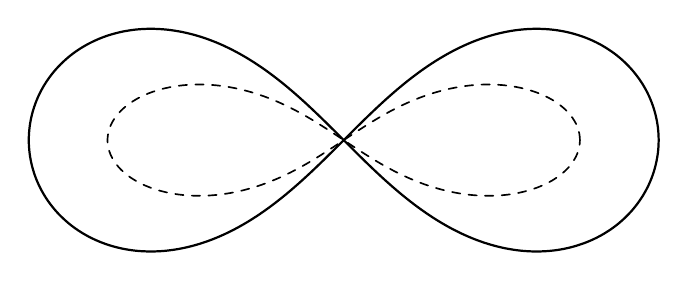
\begin{tikzpicture}[scale=2, line cap=round, line join=round]
% === Parameters for inner curve scaling ===
\def\sx{0.75} % inner horizontal scale
\def\sy{0.5}  % inner vertical scale

% === Outer solid lemniscate ===
\draw[line width=0.8pt, samples=300, domain=0:360, smooth]
  plot ({2*cos(\x)/(1+sin(\x)^2)}, {2*sin(\x)*cos(\x)/(1+sin(\x)^2)});

% === Inner dashed lemniscate (scaled) ===
\draw[dashed, line width=0.6pt, samples=300, domain=0:360, smooth]
  plot ({\sx*2*cos(\x)/(1+sin(\x)^2)}, {\sy*2*sin(\x)*cos(\x)/(1+sin(\x)^2)});
\end{tikzpicture}%
}
\end{center}